\section{Model development}

%------------------------------------------------

\begin{frame}
    \frametitle{Data scaling and resampling}
    \vspace{3mm}

	\begin{itemize}
	        \item \textbf{Data Scaling:}
	        \begin{itemize}
	            \item The radiomic features were standardized using \texttt{StandardScaler} to ensure a mean of zero and a standard deviation of one.
	            \item This prevents features with larger magnitudes from disproportionately influencing the model’s performance.
	        \end{itemize}
	
	        \vspace{3mm}
	        \item \textbf{Data Resampling:}
	        \begin{itemize}
	            \item \textbf{Undersampling:} The Luminal A class was reduced to 30 instances to decrease its dominance in the dataset.
	            \item \textbf{SMOTE (Synthetic Minority Oversampling Technique):} New synthetic samples were generated for minority classes to improve class balance.
	        \end{itemize}
	    \end{itemize}

	   \begin{figure}[h]
	        \centering
	        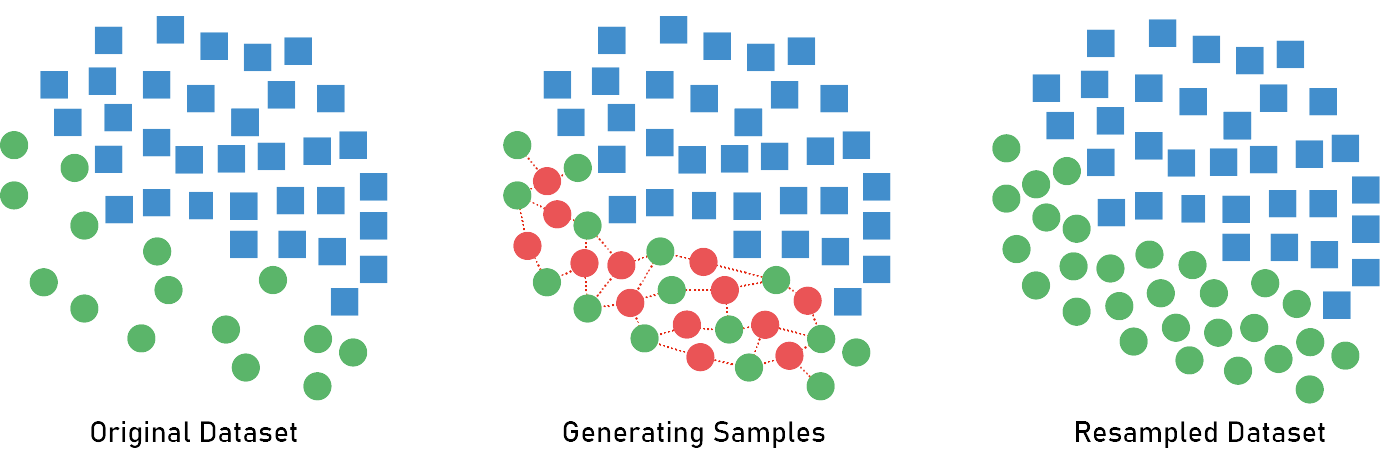
\includegraphics[width=0.75\linewidth]{smote.png}
	    \end{figure}

    \vfill 
\end{frame}

%------------------------------------------------

\begin{frame}
    \frametitle{Radiomic features-based model - Pipeline}
    \vspace{3mm}

	   \begin{figure}[h]
	        \centering
	        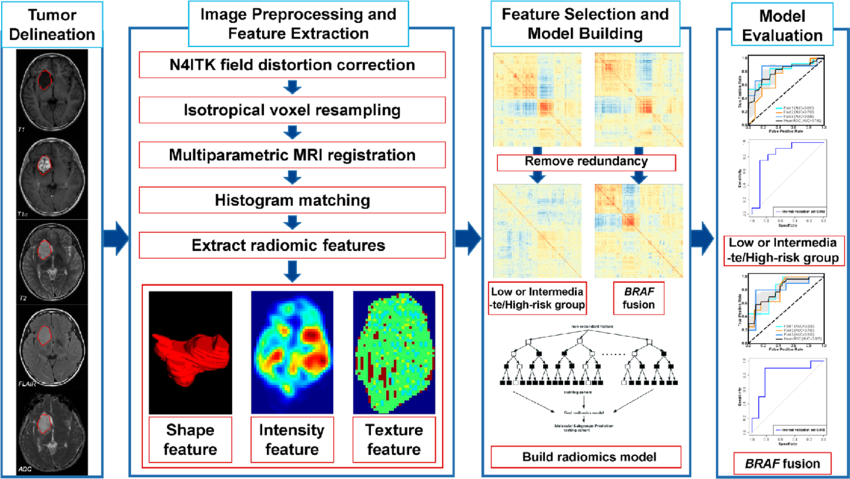
\includegraphics[width=0.75\linewidth]{radiomic_pipeline.png}
	    \end{figure}

	\vspace{2mm}
    	\begin{center}
    	In this project, we start with the given radiomic features, so feature selection and model training are yet to be performed.
	\end{center}

    \vfill 
\end{frame}

%------------------------------------------------

\begin{frame}
    \frametitle{Radiomic features-based model - Feature Selection I}
    \vspace{3mm}
	\textbf{Feature selection steps:}
    \vspace{2mm}
    \begin{itemize}
        \item \textbf{Boruta with Gradient Boosting:}
        \begin{itemize}
            \item Applied to identify the most relevant radiomic features.
            \item Reduced the feature set from 36 to 11 variables.
        \end{itemize}

        \vspace{2mm}
        \item \textbf{Redundancy Analysis:}
        \begin{itemize}
            \item \textbf{Correlation Heatmap (\ref{fig:correlation_heatmap}):} Displayed pairwise correlations between the selected features, highlighting highly correlated pairs, indicating redundancy.
            \item \textbf{Hierarchical Clustering (\ref{fig:dendrogram}):} Visualized using a dendrogram to group correlated features into clusters based on correlation distances.
        \end{itemize}
    \end{itemize}

    \vfill 
\end{frame}

%------------------------------------------------

\begin{frame}
    \frametitle{Redundancy Analysis - Correlation Heatmap}

    \begin{figure}[h]
        \centering
        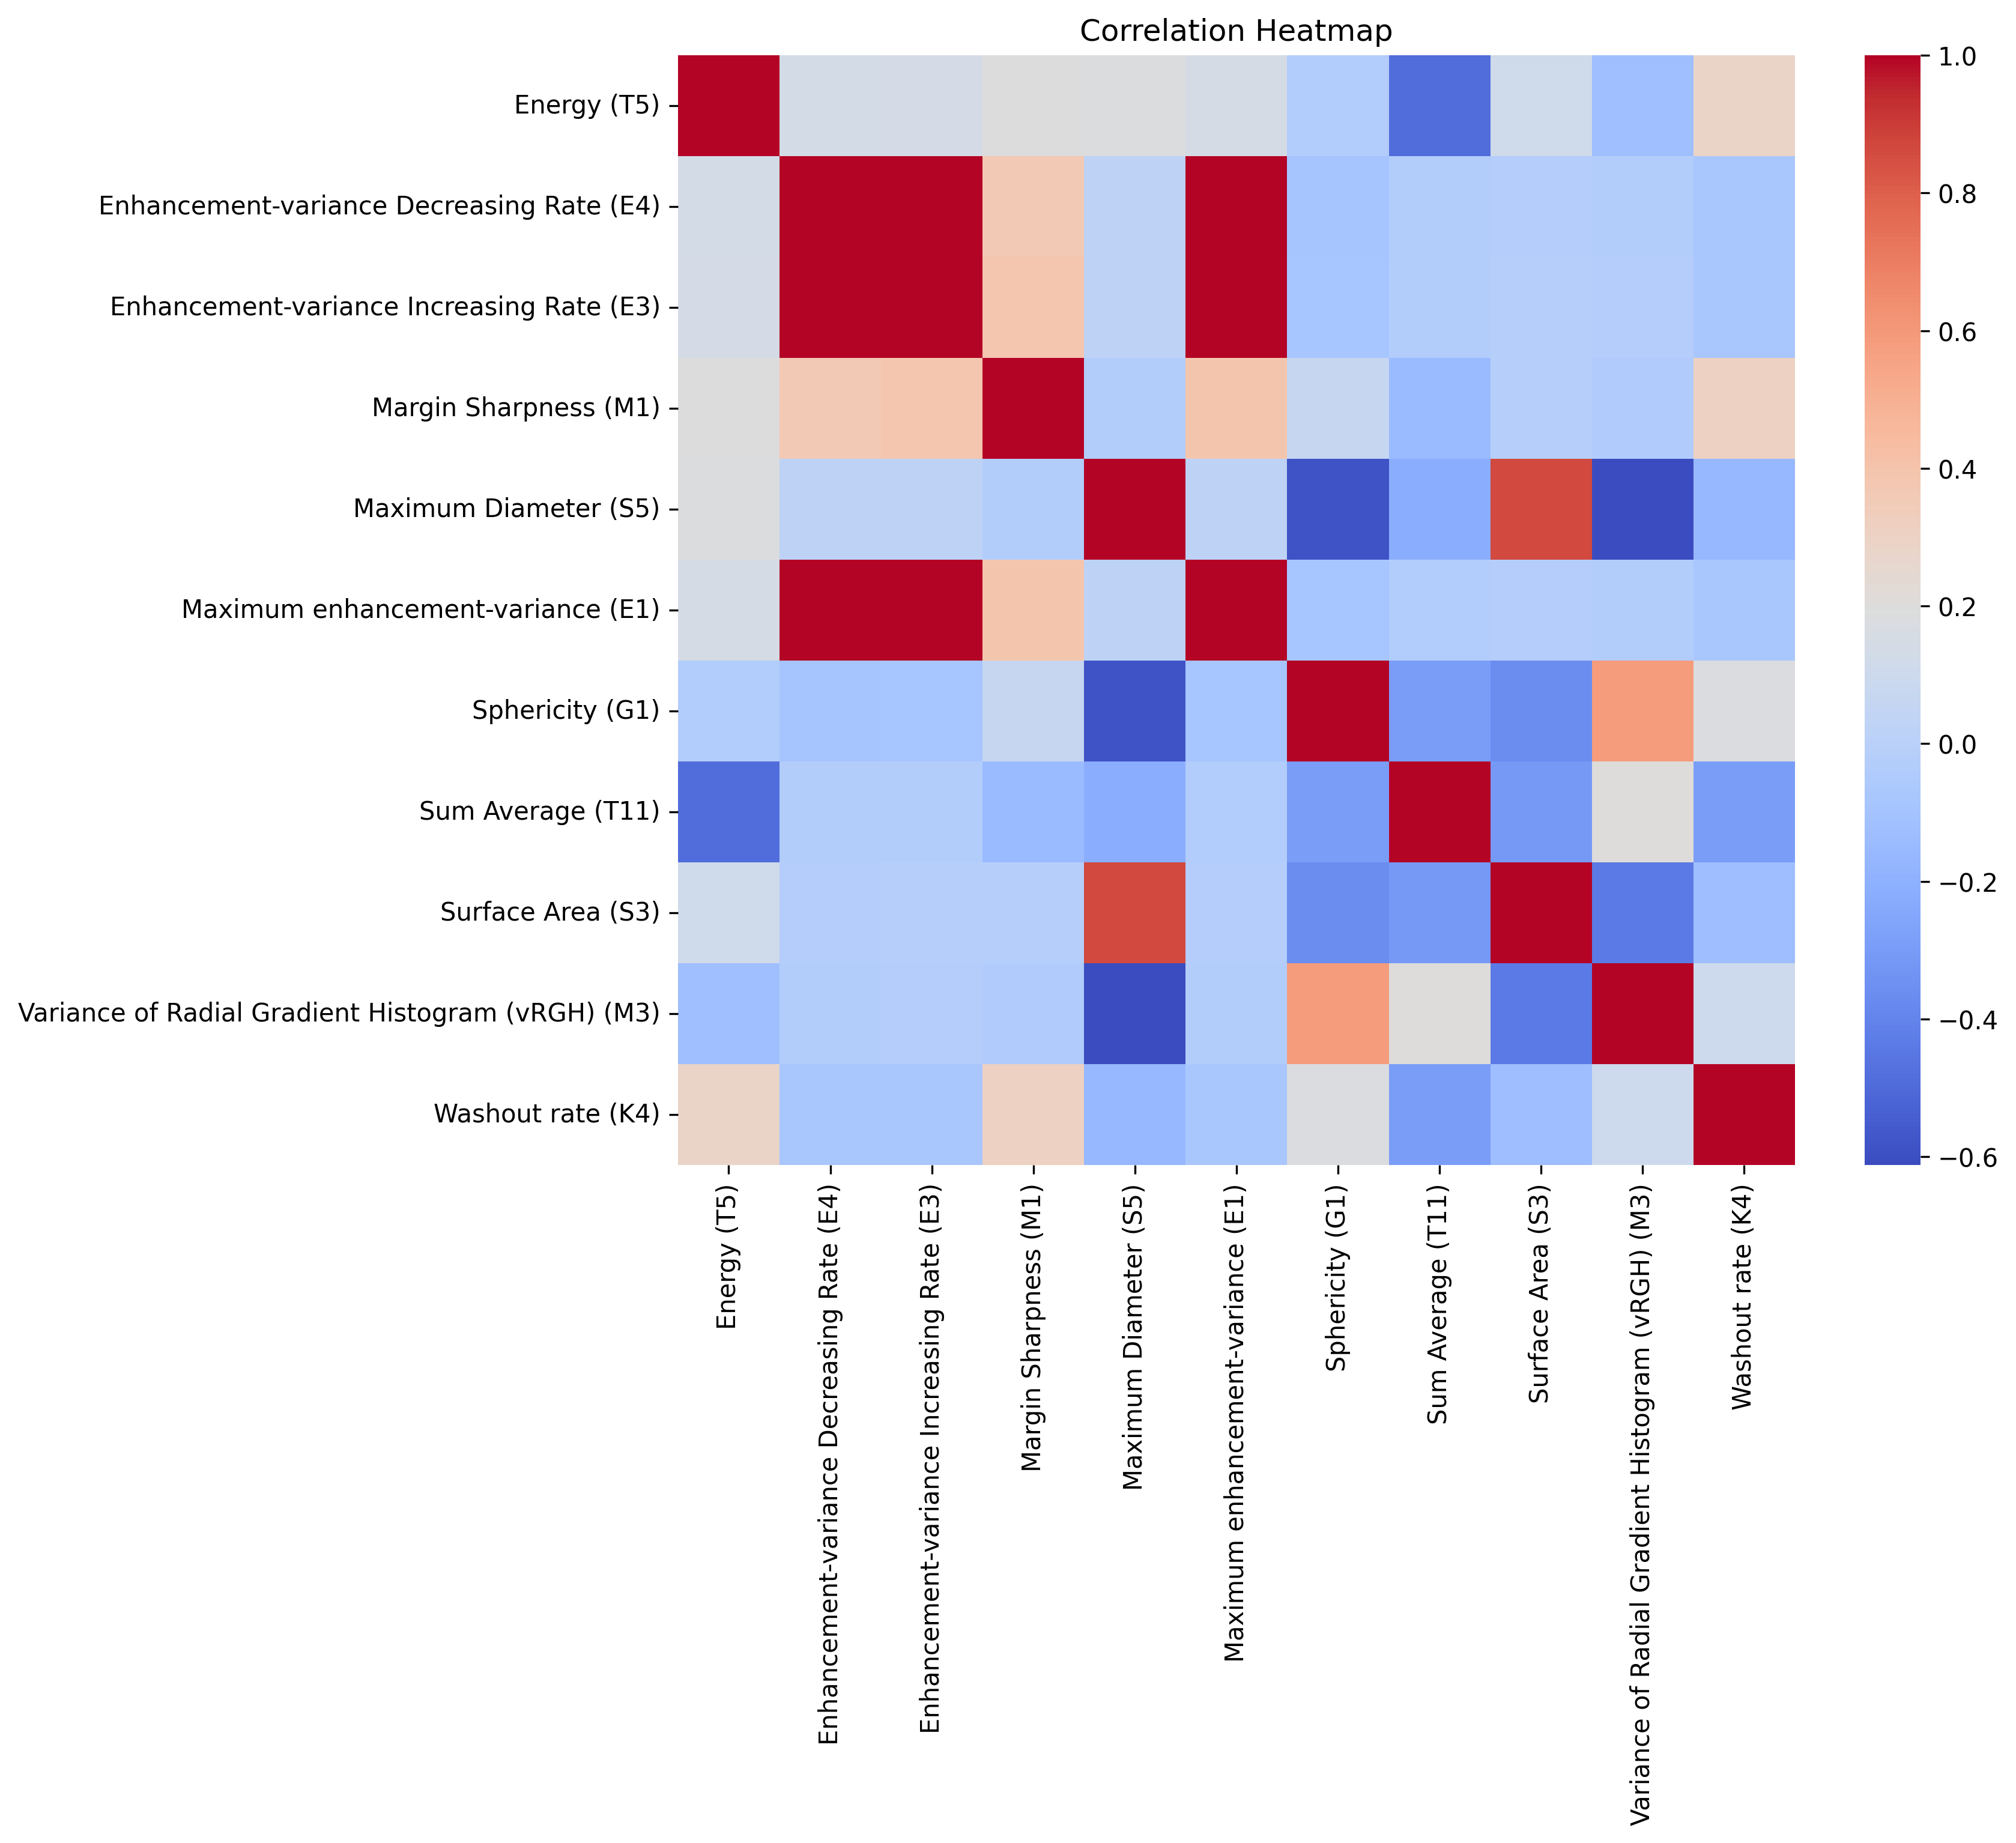
\includegraphics[width=0.7\linewidth]{correlation_heatmat.png}
        \label{fig:correlation_heatmap}
    \end{figure}

    \vfill 
\end{frame}

%------------------------------------------------


\begin{frame}
    \frametitle{Redundancy Analysis - Dendrogram}

    \begin{figure}[h]
        \centering
        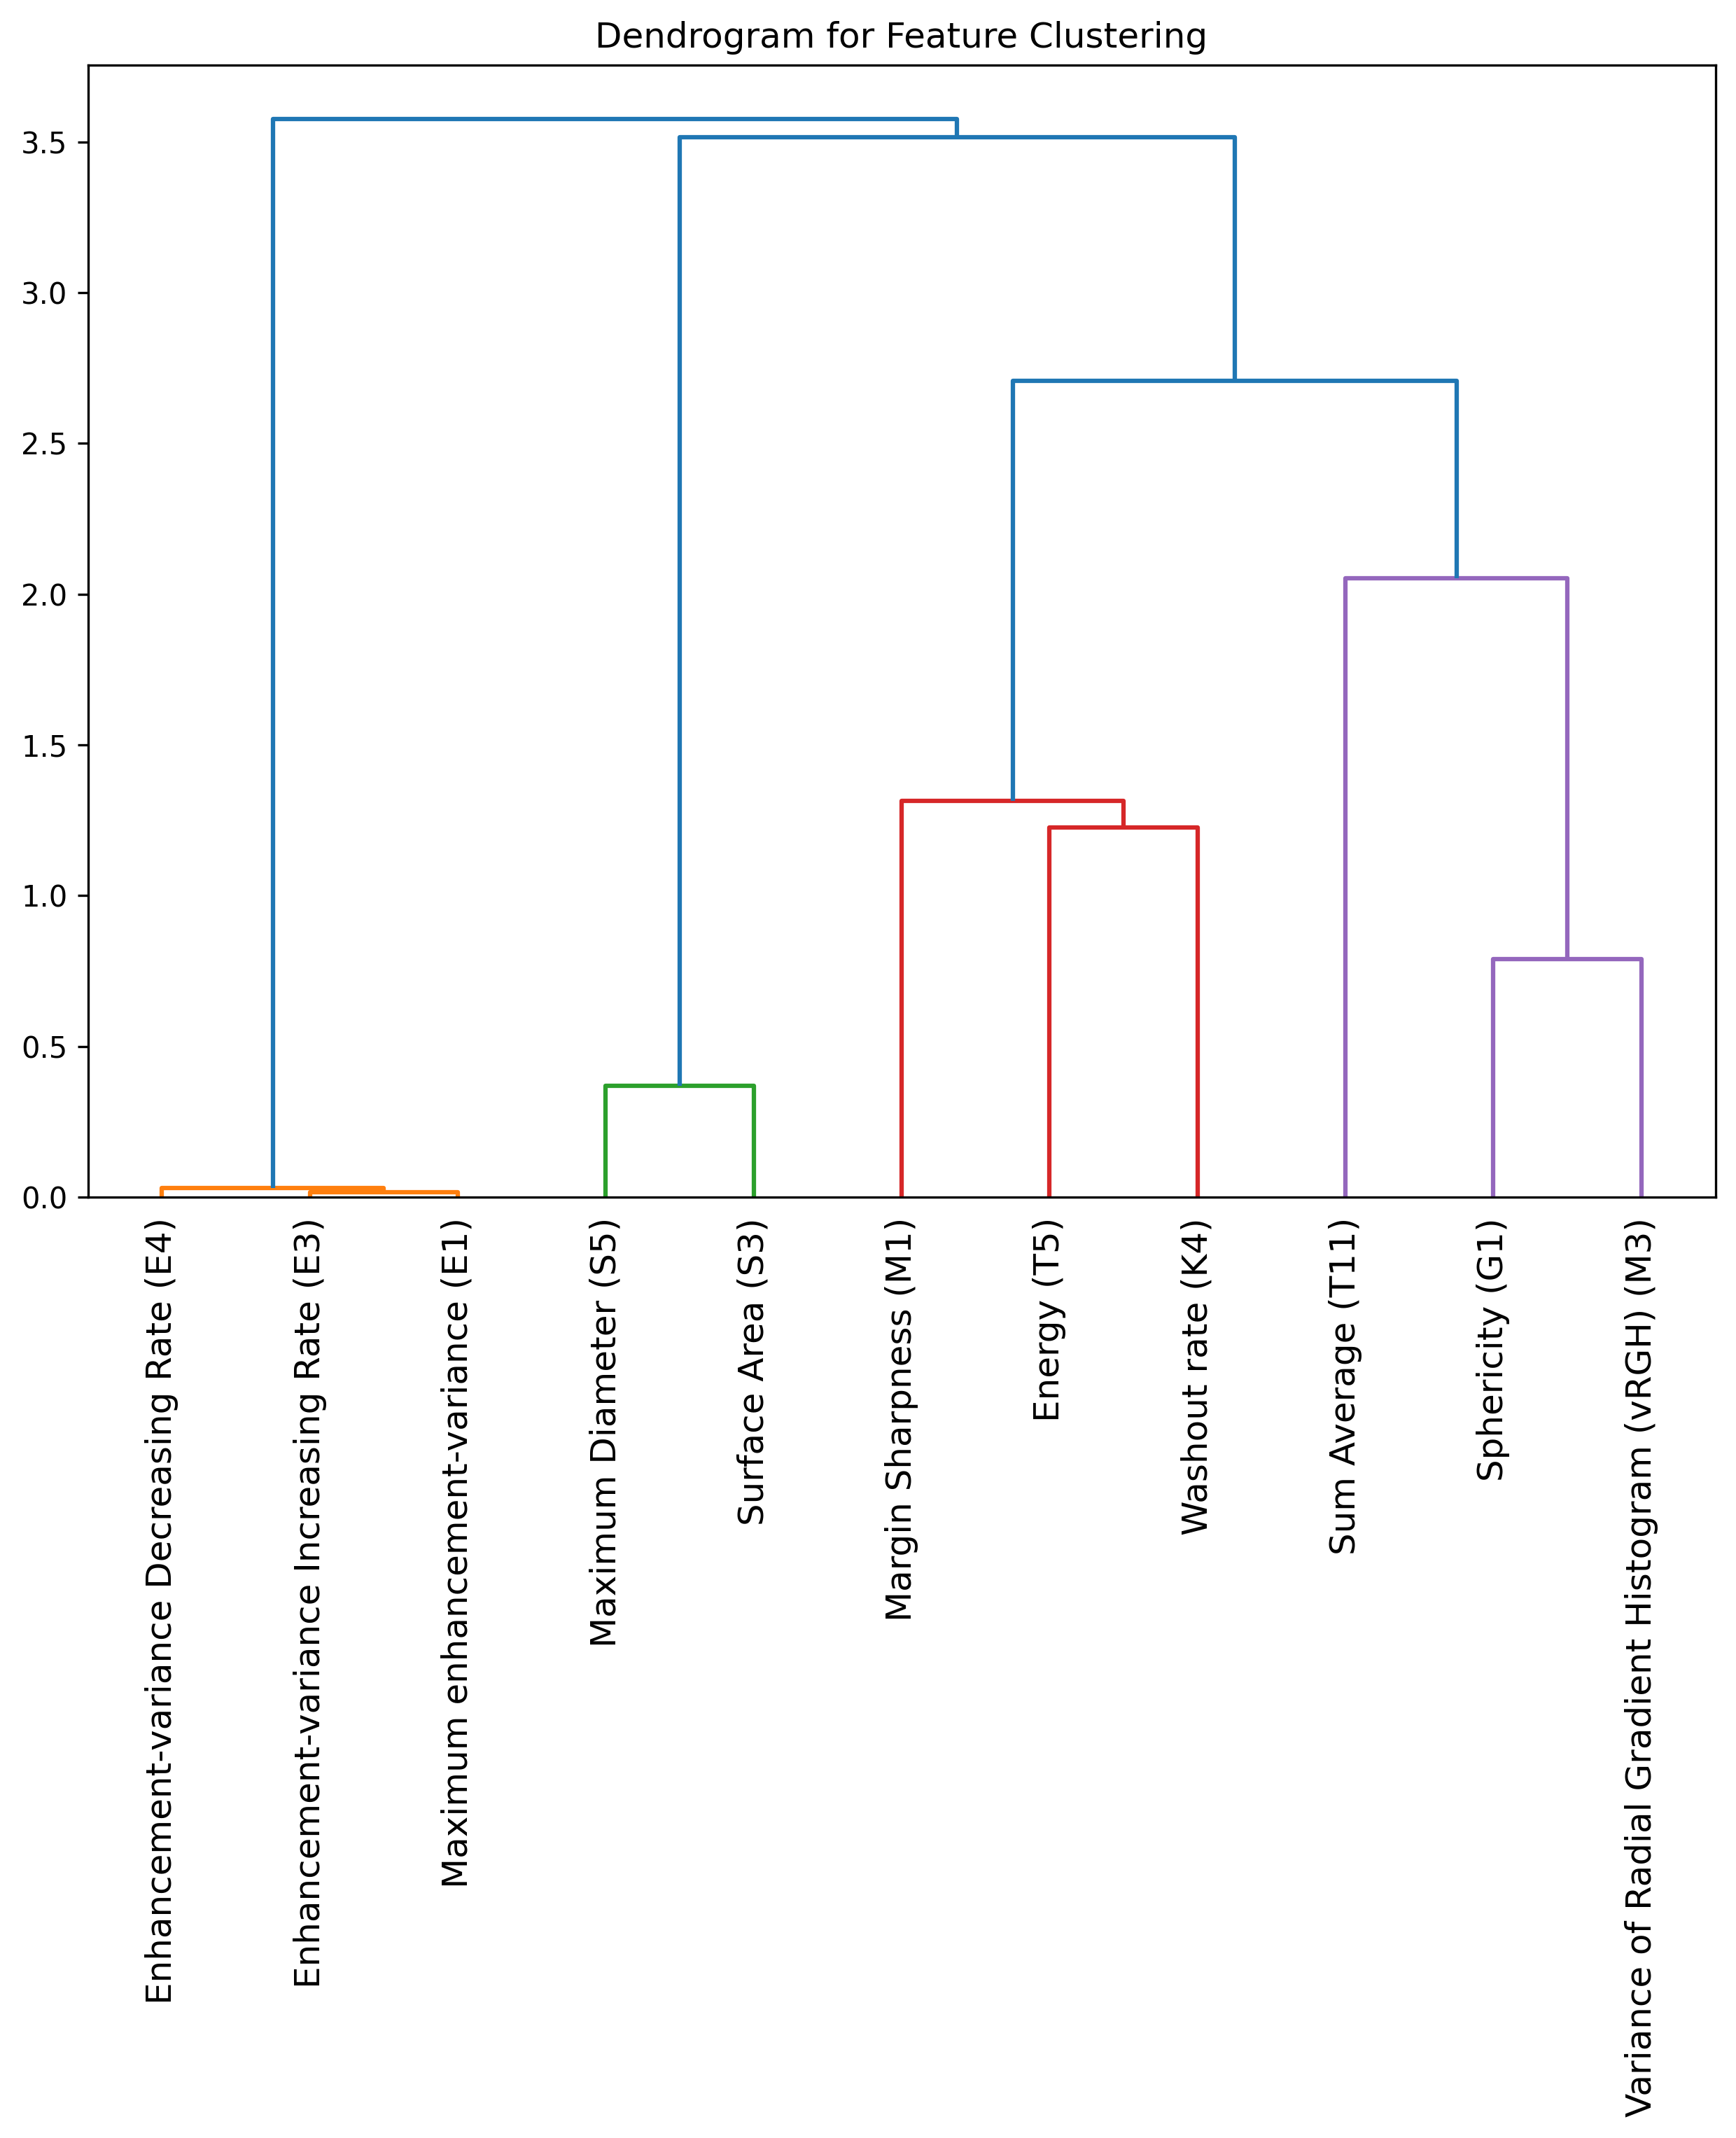
\includegraphics[width=0.525\linewidth]{dendrogram.png}
        \label{fig:dendrogram}
    \end{figure}

    \vfill 
\end{frame}

%------------------------------------------------

\begin{frame}
    \frametitle{Radiomic features-based model - Feature Sel.  II}
    \vspace{3mm}

       After testing different numbers of clusters, selecting 3 clusters provided a good balance between reducing redundancy and maintaining model performance.

                \vspace{3mm}

	\textbf{Final representative features:}
            \begin{itemize}
                \item \textbf{Margin Sharpness (M1):} Describes the abruptness of intensity changes at the tumor’s boundary, indicating how clearly the tumor is demarcated from surrounding tissue.
                \item \textbf{Maximum Enhancement-Variance (E1):} Measures the variance in the enhancement signal across the most enhancing regions, reflecting vascular heterogeneity.
                \item \textbf{Surface Area (S3):} Represents the surface area of the tumor boundary, indicating tumor size and shape complexity.
            \end{itemize}

    \vfill 
\end{frame}

%------------------------------------------------

\begin{frame}
    \frametitle{Radiomic features-based model - Model training}
    \vspace{3mm}
	
	\textbf{Once the features are selected, we train a Random Forest (RF) model.}
    \vspace{1mm}
    \begin{figure}[h]
        \centering
        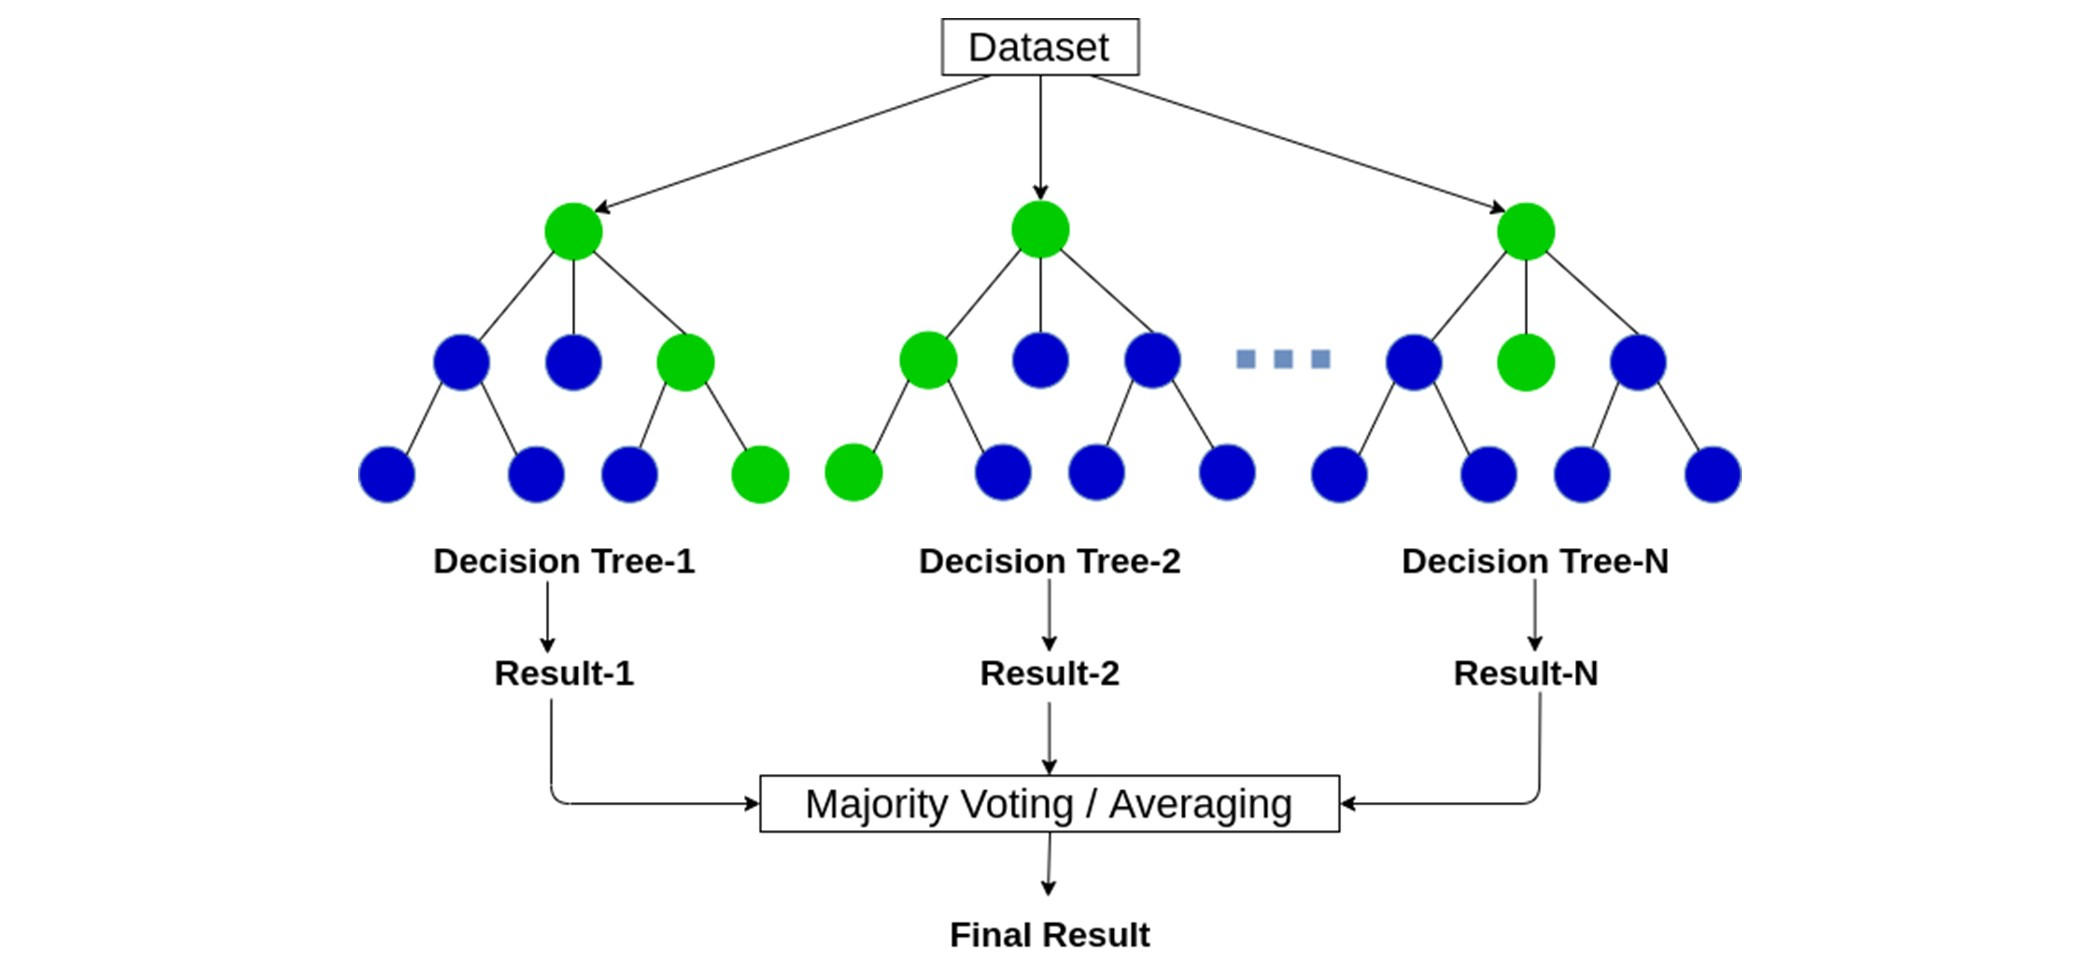
\includegraphics[width=1\linewidth]{random-forest.jpg}
    \end{figure}

    \vfill 
\end{frame}

%------------------------------------------------

\begin{frame}
    \frametitle{Radiomic model with aditional data}
    \vspace{3mm}
	
    \begin{itemize}
        \item \textbf{Radiomic Model with Clinical Data:}  
        Adds to the previous radiomic features the following variables:

	\vspace{2mm}

        \begin{itemize}
            \item \textbf{Full Clinical Data Model:}
            \begin{itemize}
                \item Age at diagnosis
                \item Cancer stage and tumor size
                \item Number of affected lymph nodes
                \item Hormone receptor status
            \end{itemize}
            \item \textbf{Reduced Clinical Data Model:}  
            This model excludes the hormone receptor status variables to avoid an overly optimistic evaluation.
        \end{itemize}

        \vspace{3mm}

        \item \textbf{Radiomic Model with Multigenic Assays:}  
        Adds to the previous radiomic features the following variables:
        \begin{itemize}
            \item GHI RS Score
            \item Correlation with good outcome signature
            \item Proliferation-related gene expression
        \end{itemize}
    \end{itemize}

    \vfill
\end{frame}